\section{Spoofing}
\label{sec:spoofing}
The spoofing was tested using different spoofing delay and positions, starting it after 300 seconds.
\subsection{Spoofing without delay}
\label{spoofing_without_delay}
We simulated spoofing using open sky measurement and a spoof position far from the receiver one.
\begin{lstlisting}
spoof.active = 1; 
spoof.delay = 0; 
spoof.t_start = 300; 
spoof.position=[41.889515,12.491858,100]+1e-3; 
\end{lstlisting} 
If we look at the pseudoranges values over time in figure \ref{fig:delay0_far} we can observe a significant change and this is caused by the high distance between the spoofed position and the receiver's one.

\begin{figure}[!htb]
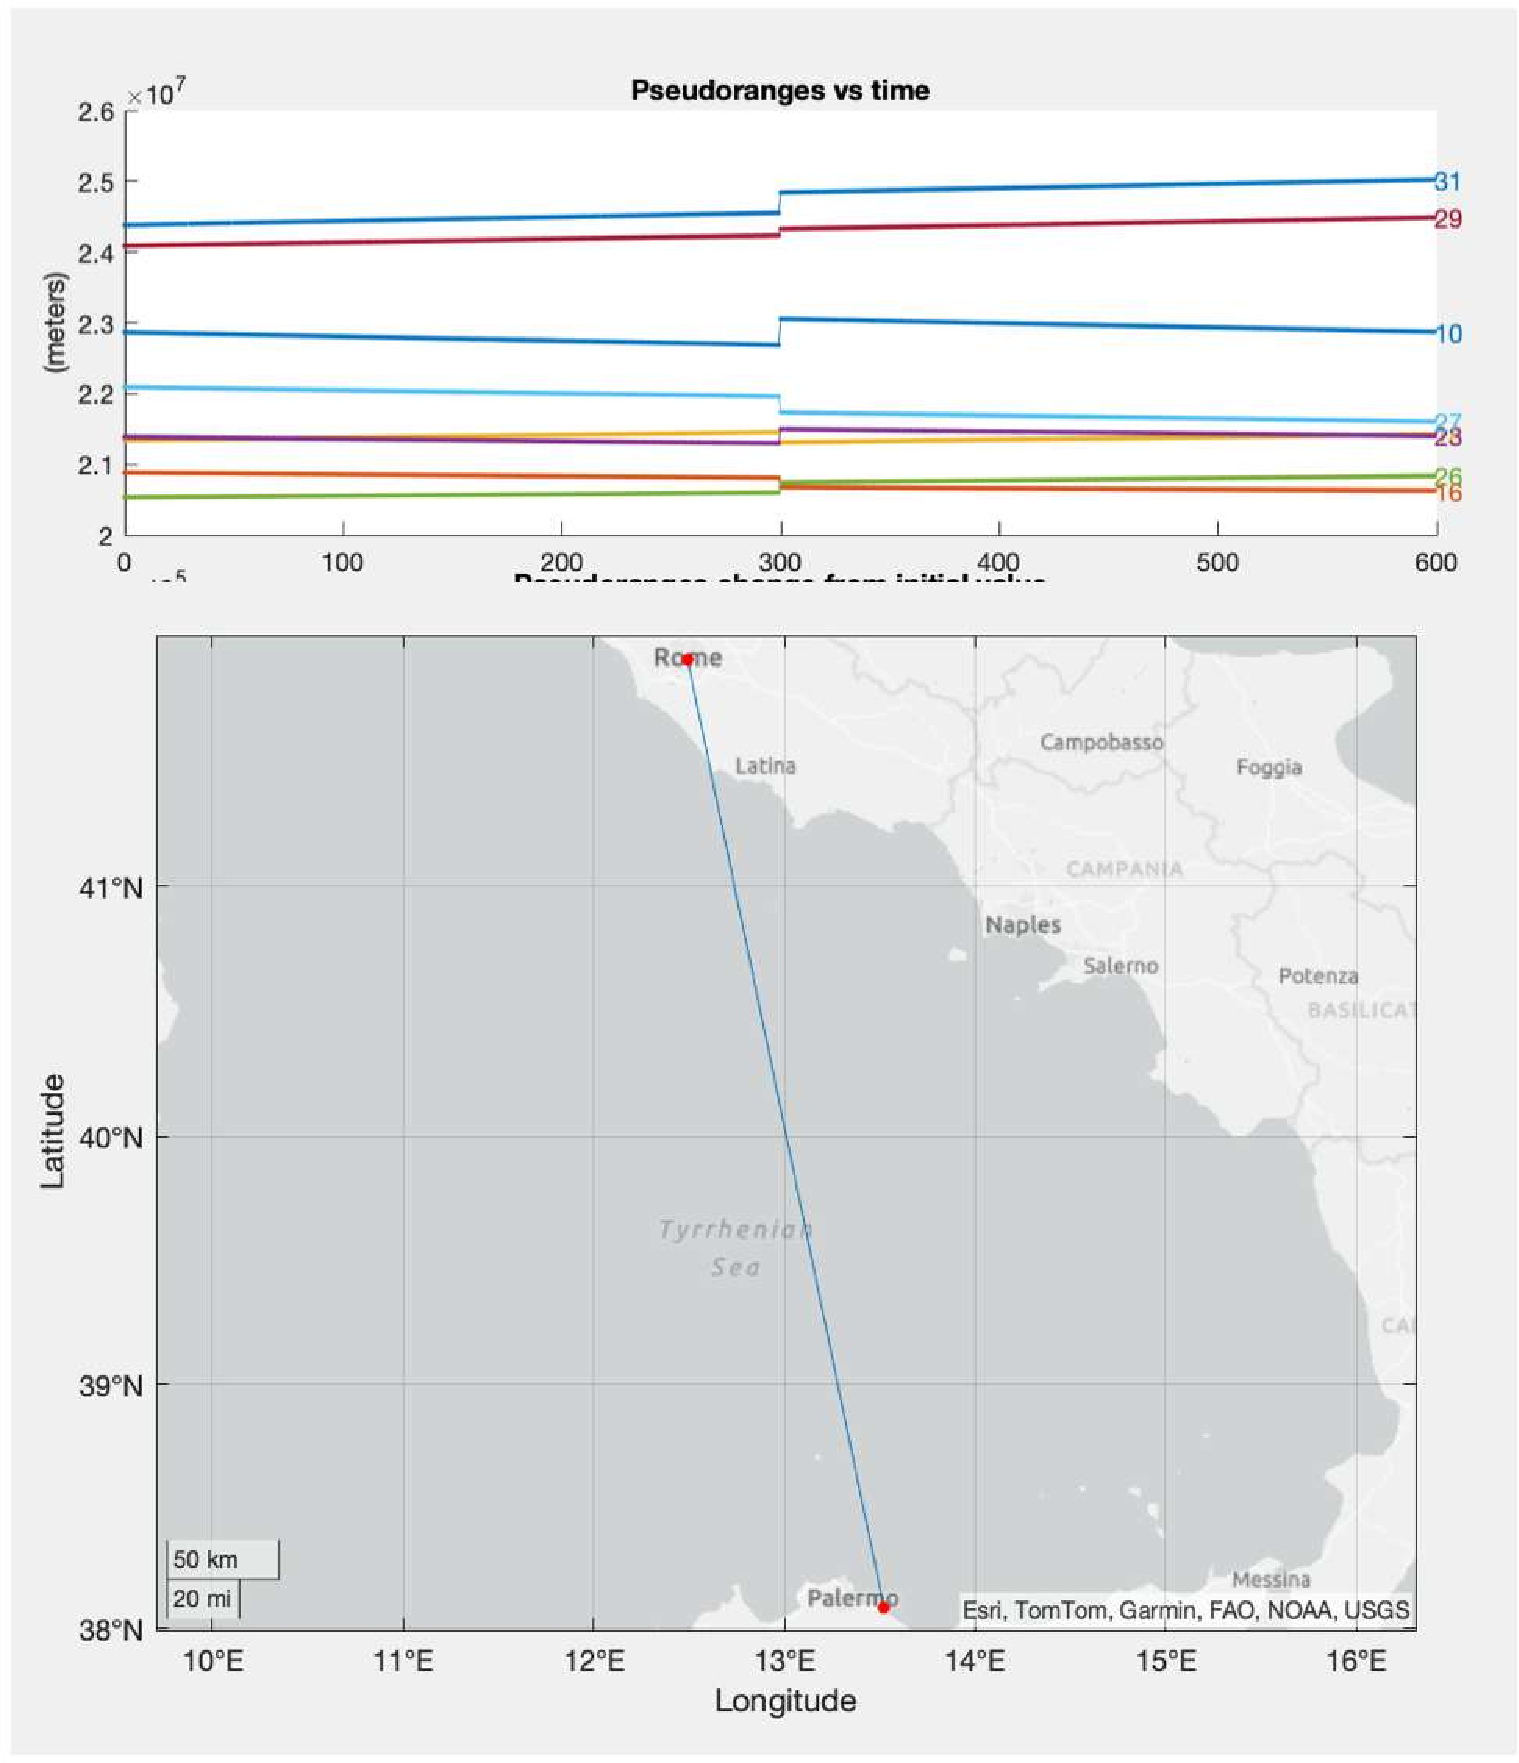
\includegraphics[scale=0.21]{images/delay0_far_figure_1_4.pdf}
\caption{Pseudoranges, positioning solution on map}
\label{fig:delay0_far}
\end{figure}

\subsection{Spoofing position near receiver}
\label{spoof_near_receiver}
In this case the spoofed position is near the receiver's one (the offset is $10^{-3}$). In figure \ref{fig:delay0}, we can observe that the change in pseudoranges over time is negligible. This is because the scale of the plot, which is on the order of $10^{7}$, makes it difficult to detect small changes, especially when compared to scenarios where the spoofed position is distant from the receiver's actual position (\ref{spoofing_without_delay}). The position estimate plot shows the real position estimated before spoofing and the fake one estimated after spoofing.

\begin{figure}[!htb]
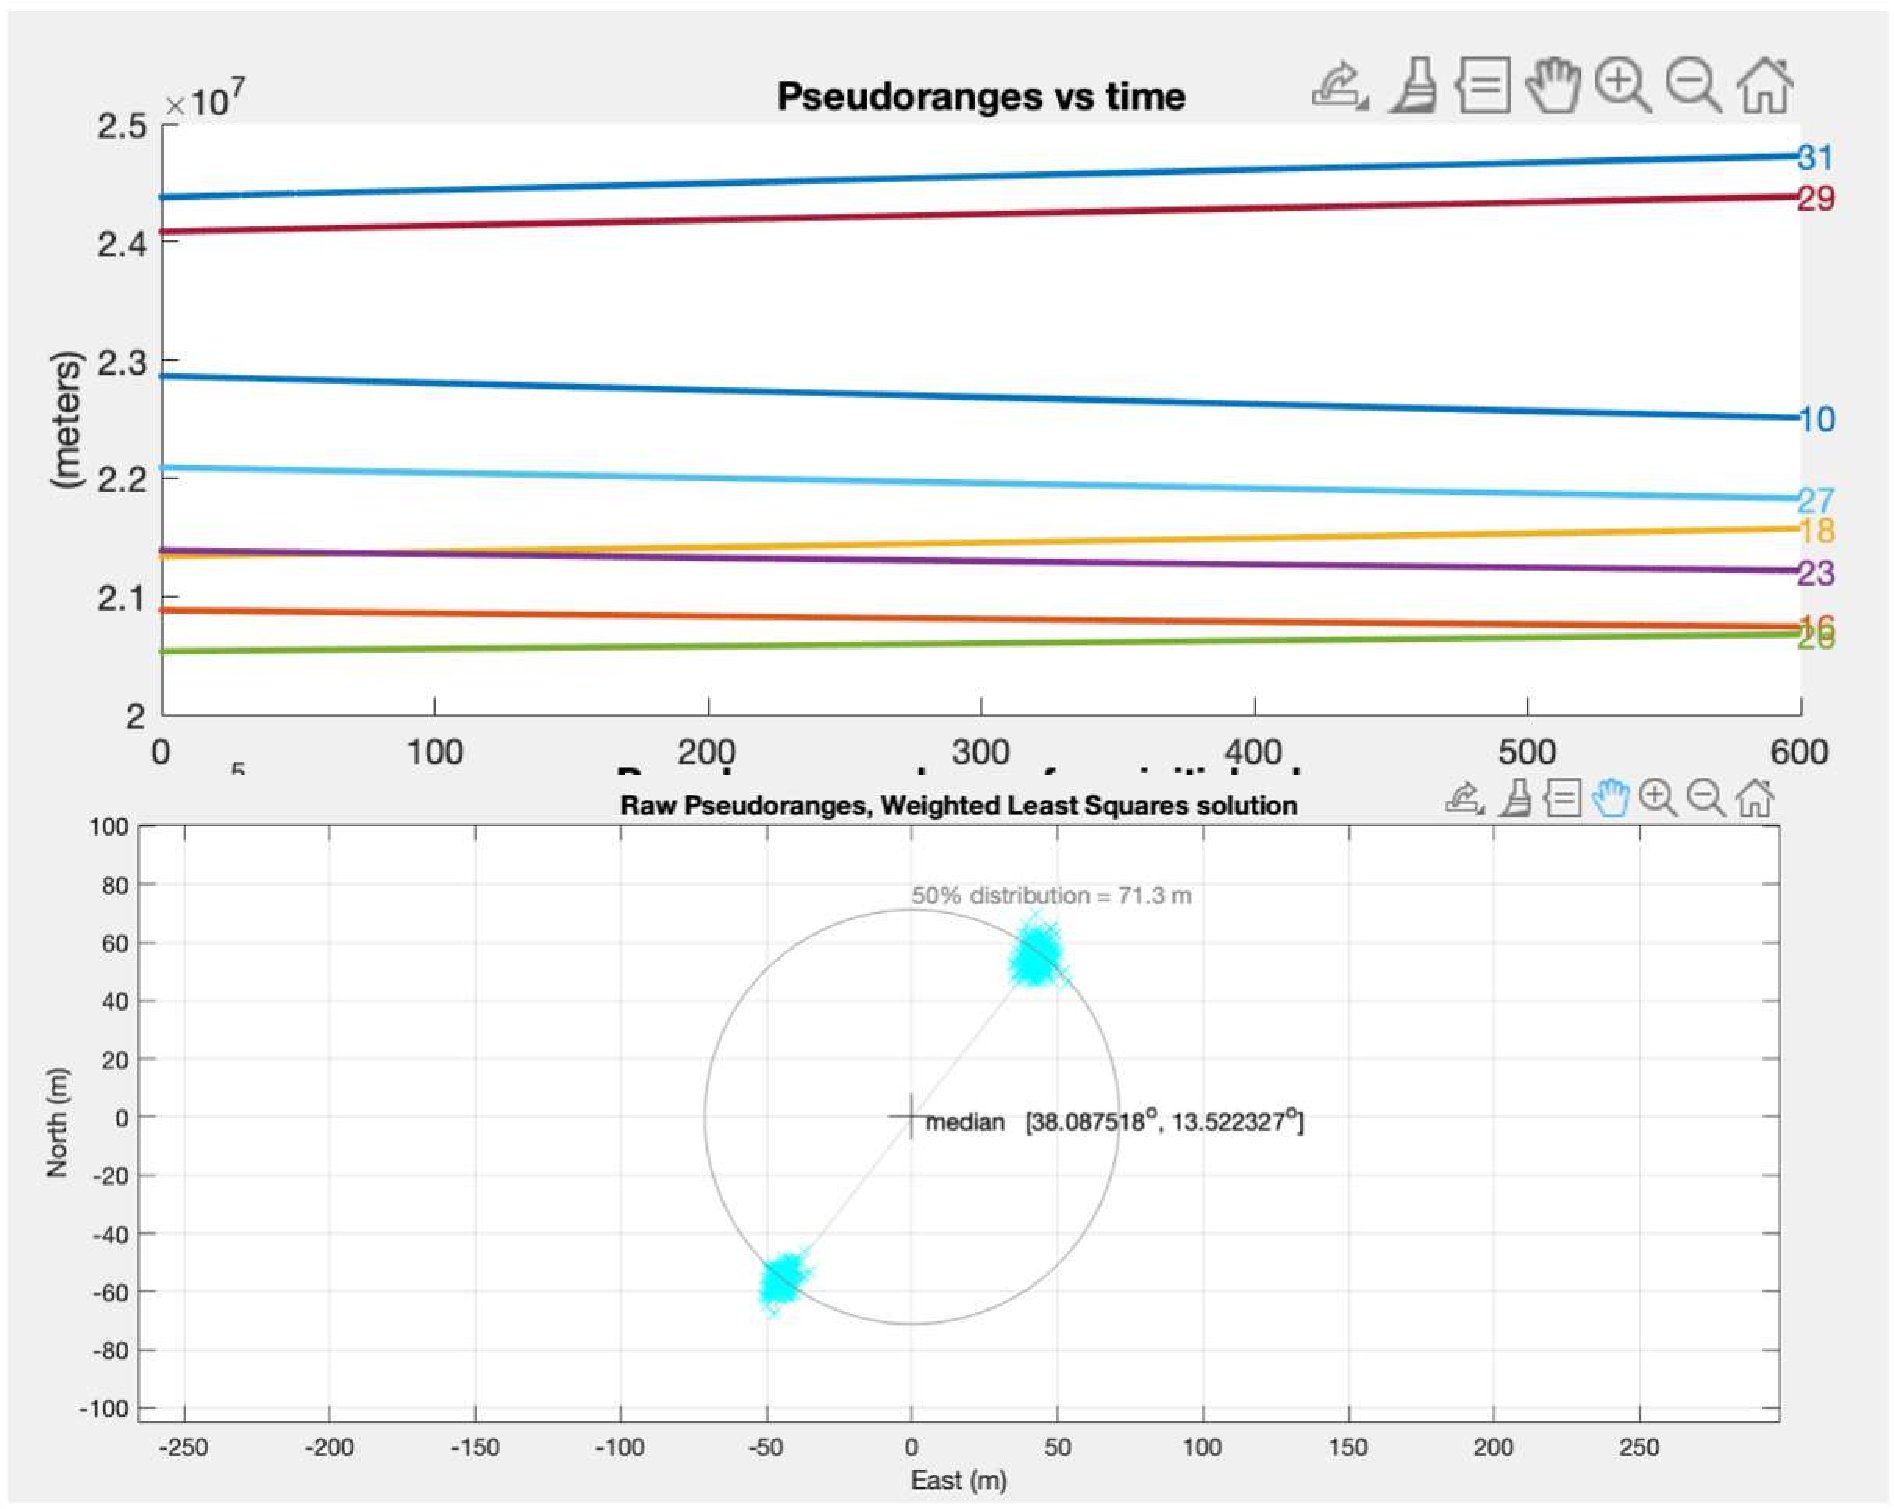
\includegraphics[scale=0.18]{images/delay0_figure_1_4.pdf}
\caption{Pseudoranges, position estimate}
\label{fig:delay0}
\end{figure}

\subsection{Spoofing with delay}
In this case, we introduce a spoof delay of 5 milliseconds, which differs from the previous scenario. Figure \ref{fig:delay0_figure_1} illustrates that the pseudoranges exhibit a peak due to our introduced spoof delay. The peak occurs because the pseudoranges are calculated based on the time of flight (the time it takes for the signal sent by the satellite to reach us), which is influenced by the receiving timestamp that is modified by our introduced delay. However, it's important to note that this delay does not impact the position estimation directly, as it is perceived as an additional clock bias. This bias is estimated by the receiver as part of its clock offset estimation process. In figure \ref{fig:delay0_figure_5_comparison}, we compare the user clock bias with and without the spoof delay and we can notice that in the former case there is a peak corresponding to the initiation of the spoofing.

\vspace{2cm}
\begin{figure}[!htb]
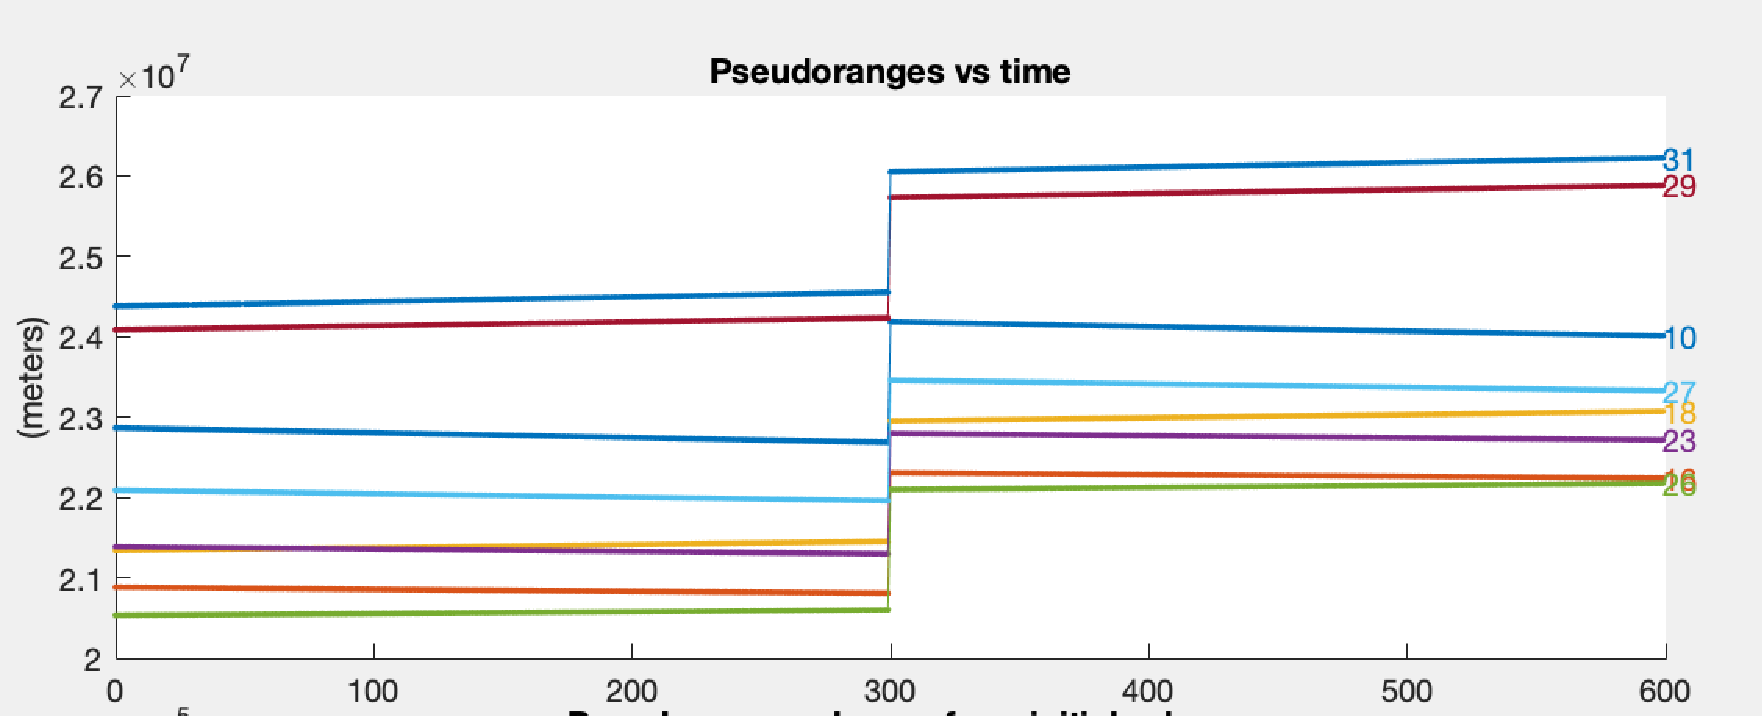
\includegraphics[scale=0.2]{images/delay_figure_1.pdf}
\caption{Pseudoranges}
\label{fig:delay0_figure_1}
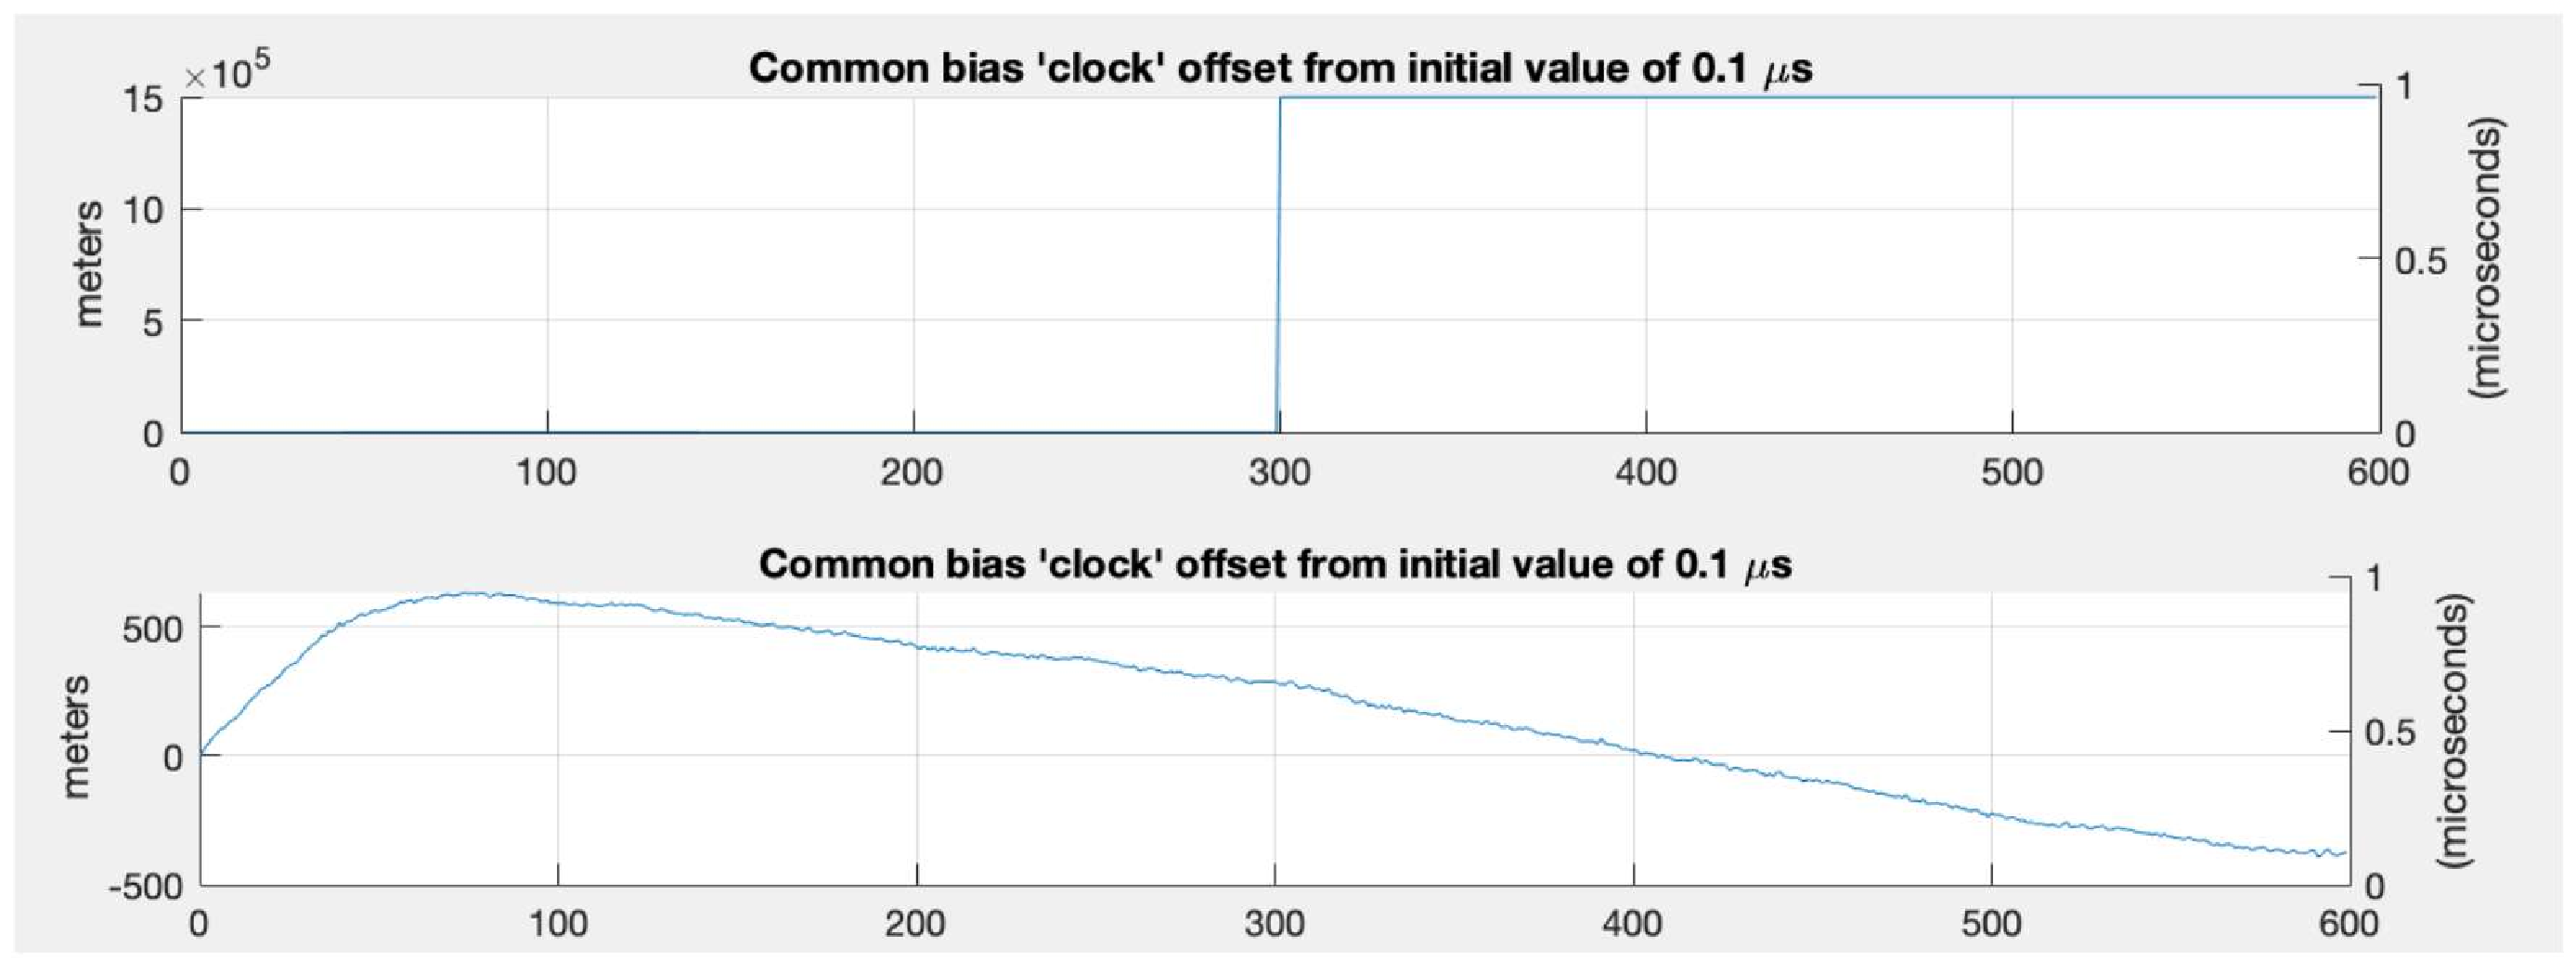
\includegraphics[scale=0.15]{images/delay_figure_5_comparison.pdf}
\caption{Clock bias difference between delayed and non-delayed}
\label{fig:delay0_figure_5_comparison}
\vspace{15pt}
\end{figure}
\vspace{-20pt}
\subsection{Spoofing detection}
\label{subsec:spoofing_detection}
One way to detect spoofing attack is to observe the pseudoranges variation over time because, as we have previously seen, if the spoofed position is far from the real receiver one, or if the spoofer transmit the signals with a delay, the pseudoranges changes rapidly. If this change is greater than a reasonable threshold we can assume that the attack is underway. Another possible detection method is based on the carrier to noise ratio: if the spoofer does not transmit the signals with a power similar to a real satellite, then it's possible to detect that it is a fake signal. Moreover, it is possible to verify if the received signals originates from satellites that are really in view of the receiver or they are just fake signal generated by the spoofer for example by using cryptographic techniques or by analyzing the receiving direction (this can be done if we have an antenna which is able to tell you the signal direction of arrival).